As discussed in Chapter \ref{chap:intro}, the search of the Standard Model Higgs boson decaying to bottom quarks is essential in confirming the properties and the nature of the Higgs boson. The most sensitive production channel to study \Hbb is Vector Boson Associated (VH) production, as the requirement of having leptons or missing energies in the final state can reduce the background significantly. Most of the previous attempts to measure \Hbb were through the VH channel. Collaboratively, the CDF and D0 experiments measured the \Hbb signal strength to be $\mu=\sigma/\sigma_\text{SM}=1.9 \pm 0.8$ ~\cite{Aaltonen:2012qt}. In the LHC era, Run I and early Run II combination of ATLAS and CMS experiments measured $\mu=0.90 \pm 0.27$ with a $3.6\sigma$ observed significance~\cite{HIGG-2016-29} and $\mu=1.1 \pm 0.3$ with a $3.8\sigma$ observed significance~\cite{CMS-HIG-16-044} respectively.

The Vector Boson Fusion (VBF) production mode serves as an orthogonal and complementary channel to the VH production, as the final states of the VBF \Hbb process are fully hadronic. Compared to Gluon-Gluon Fusion (ggF) production mode, which also has fully hadronic final states but look very similar to generic multi-jet QCD processes, the VBF production has special event topologies which can be exploited to suppress the QCD background. Since the Higgs bosons are color singlets with no color connection from other leading order final state particles to the decay product bottom quarks; little QCD radiation and hadronic activity is expected between the VBF jets, creating a rapidity gap between them (Fig. \ref{fig:vbf-feynman}).

\begin{figure}[htpb!]
\begin{center}
  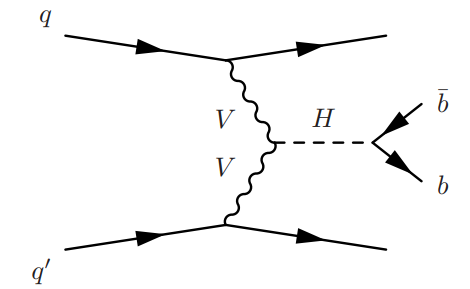
\includegraphics[width=0.55\linewidth]{figures/VBF/VBFFeynman.png}
\caption{Feynman diagram for VBF \Hbb process}
\label{fig:vbf-feynman}
\end{center}
\end{figure}


Using 20.2 \ifb~of data from 8~\tev~collisions, the ATLAS experiment measured a yield of -0.8$\pm$2.3 times the Standard Model predicted value\cite{HIGG-2014-12}. The CMS Collaboration released a result\cite{CMS-HIG-14-004} at \rts=8~\tev, and observed a fitted signal strength of $\mu = \sigma/\sigma_{SM} = 2.8^{+1.6}_{-1.4}$, corresponding to an observed significance of 2.2 standard deviations.   From combined measurements by both the ATLAS and CMS experiments\cite{HIGG-2015-07}, the measured signal strength for VBF production and the Higgs coupling to bottom quarks are $\mu_{\rm VBF}({\rm ATLAS+CMS})  = 1.18_{+0.25}^{-0.23}$ and $\mu_{bb} ({\rm ATLAS+CMS}) = 0.70^{+0.29}_{-0.27}$, respectively. The Run I VBF \Hbb results from both experiments are not very sensitive and conclusive and demonstrates the need of a continued study of this process. Due to the increase of the center of mass energy for the Run II LHC operation, the theoretical VBF Higgs production cross-section for mass at 125 \GeV increases by a factor of 2.3 from 8 to 13~\tev leading to a potentially more sensitive analysis than Run I. 

The overall strategy of the Run II VBF \Hbb analysis is fairly similar to that of Run I. The VBF \Hbb events have two $b$-jets and two VBF jets in the final states. Therefore, the event pre-selection starts from tagging two $b$-jets and requiring the events to have two more non $b$-tagged jets as documented in Sec.\ref{sec:vbf-objsel}. Two sets of the triggers specifically target for two different topologies in which either the two VBF jets are in the central region of the detector (\fourcentral channel) or at least one VBF jet is in forward region (\twocentral channel) as described in Sec.\ref{sec:vbf-evtsel}. As shown in ~\cite{HIGG-2014-12}, Boosted Decision Tree (BDT) based analysis yields better overall sensitivity than cut-based analysis. This analysis adopted the BDT method to find most sensitive phase space to extract Higgs signal as described in Sec.\ref{sec:vbf-bdt}. The BDT is trained on simulated VBF signal events against backgrounds which are derived from data sidebands (events passing pre-selections with \Mbb in the region 80 \GeV~$< \Mbb<$~100 \GeV~ and  150 \GeV~$<$ \Mbb). The observed signal is extracted from a simultaneous fit to the \Mbb distribution in several regions defined by the event BDT scores with varying signal to background ratios. In each region, data is assumed to be the sum of non-resonant background (modeled with Bersnstein polynomials \ref{sec:vbf-nonres}), a resonant $Z$ contribution and a resonant Higgs contribution, both of which are parameterized by Bukin functions.

The Higgs mass window, i.e. the region 100 \GeV~$< \Mbb<$~140 \GeV, is kept blinded until the final profile likelihood fit is performed.  The fit strategy is validated first with a sideband-only fit to the $Z$ contributions, as described in Section~\ref{sec:vbf-zunblind}. The signal is extracted via a likelihood minimization where all relevant uncertainties are profiled and presented in Section~\ref{sec:vbf-higgsunblind}. Both the VBF process strength and the \Hbb process strength are measured. In Sec.~\ref{sec:vbf-higgscomb} the results are fit simultaneously with a related analysis (VBF$+\gamma$), the search for Higgs decays to $b$-quarks in events enriched in VBF production with the additional requirement of a photon. Finally the combination results with other \Hbb production modes are shown in Sec.\ref{sec:vbf-hbbcomb}.

The work of this chapter is published as \cite{vbfmypaper}. 


%In this analysis we cannot separate the VBF \Hbb and $ggF$ \Hbb contributions except during the BDT training, which is trained only on VBF events.  Thus all results are reported for the sum of the VBF and $ggF$ contributions.   Depending on the channel and region, the VBF and ggF contribution to the total Higgs signal varies significantly. In the most sensitive BDT regions, 81\% (\twocentral) and 82\% (\fourcentral) of the expected Higgs yield come from VBF production; while in the least sensitive regions, the ggF production dominate (77\% for \twocentral and 75\% for \fourcentral).


%This analysis is performed separately for two exclusive channels which correspond to the two trigger chains used to collect the data.  The \fourcentral channel requires four jets within $|\eta| < $2.8.  The \twocentral channel requires two central jets, and at least one jet with 4.4~$>|\eta|>$~3.2.  These channels are described in more detail in Section~\ref{sec:evtsel}. The kinematic properties of these jets are used as inputs to a boosted decision tree (BDT), described in Section~\ref{sec:bdt}.  The BDT is trained to classify events as signal-like or background-like.  

%Training signal events are taken from Monte Carlo (MC) simulation.  The background training uses events from data which pass the full event selection but have a Higgs candidate mass, \Mbb, 


